\documentclass{ctexart}
\usepackage[a4paper,total={6in,8in}]{geometry}
\usepackage{fancyhdr}
\usepackage[table,xcdraw]{xcolor}
\usepackage{diagbox}
\usepackage[utf8]{inputenc}
\usepackage{ctex}
\usepackage{color}
\usepackage{subfigure}
\usepackage{cite}
\usepackage{graphicx}
\usepackage{fontspec}
\setmainfont{Times New Roman}
\newfontfamily\timesfont{Times New Roman}
\usepackage{CJK}
\usepackage{indentfirst}
\usepackage{amsmath}
\usepackage{mathrsfs}
\usepackage{multirow}
\usepackage{svg}
\usepackage{amsfonts}
\usepackage{geometry}
\usepackage{hyperref}
\usepackage{mathabx}
\usepackage{cases}
\usepackage{minipage-marginpar}
\usepackage{xcolor}
% 导入包
\usepackage{hyperref}
% 格式设置
\hypersetup{hidelinks,
	colorlinks=true,
	allcolors=blue,
	pdfstartview=Fit,
	breaklinks=true}

\begin{document}

\begin{titlepage}
    \title{{\fontsize{28}{32}\selectfont\kaishu 机器人学 \\ \fontsize{20}{24}\selectfont\kaishu{作业5:运动学轨迹规划}}}
    \date{} % delete date as you want
    \maketitle
    \vspace{-7em}
    \begin{center}
      \fontsize{18}{22}\selectfont
      \textbf{\timesfont Robotics (2023-2024-2) \\
      Homework 5: Kinematic Trajectory Planning}
    \end{center}
    
    \begin{figure}[h]
        \centering
        
\includegraphics[width=0.45\textwidth]{Image/校标-校徽.png}
    \end{figure}
    \begin{center}
      \hspace{6em}
      \renewcommand{\arraystretch}{2}
      \begin{tabular}{rl}
      \fontsize{16}{50}\selectfont\heiti 姓名:& \fontsize{16}{24}\selectfont\heiti 赵四维 \\
      \fontsize{16}{24}\selectfont\heiti 学号:& \fontsize{16}{24}\selectfont 521021910696 \\
      \fontsize{16}{24}\selectfont\heiti 班级:& \fontsize{16}{24}\selectfont ME3403-01 \\
      \fontsize{16}{24}\selectfont\timesfont E-mail:& \fontsize{16}{24}\selectfont racheus.11@sjtu.edu.cn \\
      \end{tabular}
    \end{center}
    \begin{center}
      \fontsize{16}{24}\selectfont\timesfont \today
    \end{center}
\end{titlepage}

\pagenumbering{arabic}

\newpage
% \tableofcontents


\newpage
\pagestyle{fancy}
\fancyhf{}
\fancyhead[L]{ME3403-01}
\fancyhead[C]{机器人学Homework3}
\fancyhead[R]{赵四维 521021910696}
\fancyfoot[C]{\thepage}
\section{RRP机器人的运动学分析}
\subsection{建立MDH坐标系,并填写表格}
\begin{figure}[h]
	\centering
	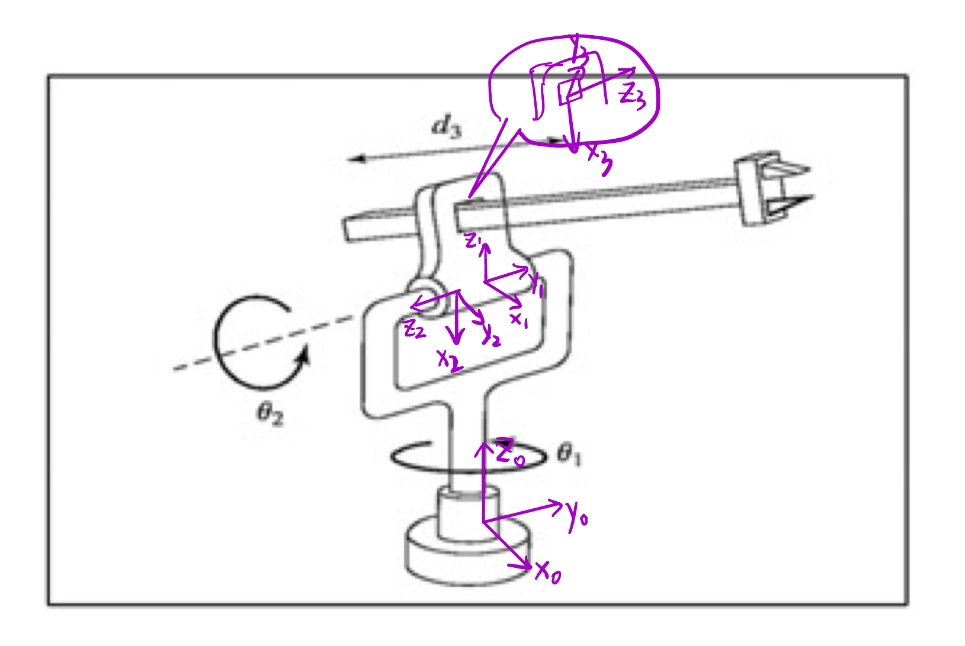
\includegraphics[width=0.6\textwidth]{Image/1.png}
	\caption{RRP机器人建系示意图}
\end{figure}

建立如上图所示的坐标系,填写MDH参数表如下,三个标蓝的参数代表输入:

\begin{table}[h]
	\centering
	\setlength{\tabcolsep}{8mm}{
	\begin{tabular}{
	>{\columncolor[HTML]{ECF4FF}}c |
	>{\columncolor[HTML]{ECF4FF}}c |
	>{\columncolor[HTML]{ECF4FF}}c |
	>{\columncolor[HTML]{ECF4FF}}c }
	\hline\hline
		\diagbox{Parameter}{Joints}	 & 1         & 2         & 3     \\ \hline
	$\theta$ &  {\color[HTML]{3531FF} $\theta_1(0^\circ)$}& {\color[HTML]{3531FF} $\theta_2-90^\circ$} & $90^\circ$     \\ \hline
	$d$      & $d_1(1)$         & 0      & {\color[HTML]{3531FF} $d_3$} \\ \hline
	$\alpha_{i-1}$ & 0         & $90^\circ$    & 0    \\ \hline
	$a_{i-1}$      & 0         & 0          & $-d_2(-0.5)$   \\ \hline\hline
	\end{tabular}}
	\caption{RRP机器人MDH参数表}
\end{table}

\subsection{写出 DH 矩阵,并使用 DH 矩阵表示机构末端相对于基座的位姿。}
由题意,逐步分析每个关节的David-Hartenberg参数:
\begin{itemize}
	\item Joint1: $\theta = \theta_1$,$a_0=0$,$d_1=1$,$\alpha_0=0$,$^0R_1=\begin{bmatrix}
		\cos\theta_1 & -\sin\theta_1 & 0 & 0 \\
		\sin\theta_1 & \cos\theta_1 & 0 & 0 \\
		0 & 0 & 1 & 1 \\
		0 & 0 & 0 & 1
	\end{bmatrix}$

	\item Joint2: $\theta = \theta_2$,$a_1=0$,$d_2=0$,$\alpha_1=90$,但是这一步的建系我始终觉得有点问题并且我查阅资料后不太知道该怎样修改。所以我决定不用表格中的参数,按照图1中的坐标关系建立旋转矩阵。
	\begin{equation}
		\begin{aligned}
		^1R_2=R_x(90)R_z(\theta_2-90)&=\begin{bmatrix}
			1 & 0 & 0 & 0 \\
			0 & 0 & -1 & 0 \\
			0 & 1 & 0 & 0 \\
			0 & 0 & 0 & 1
		\end{bmatrix}\begin{bmatrix}
			\cos(\theta_2-90) & -\sin(\theta_2-90) & 0 & 0 \\
			\sin(\theta_2-90) & \cos(\theta_2-90) & 0 & 0 \\
			0 & 0 & 1 & 0 \\
			0 & 0 & 0 & 1
		\end{bmatrix}
		\\&=
		\begin{bmatrix}
			\cos(\theta_2-90) & -\sin(\theta_2-90) & 0 & 0 \\
			0 & 0 & -1 & 0 \\
			\sin(\theta_2-90) & \cos(\theta_2-90) & 0 & 0 \\
			0 & 0 & 0 & 1
		\end{bmatrix}
	\end{aligned}
	\end{equation}
	\item Joint3: $\theta=90^\circ$,$a_2=-0.5$,$d_3=d_3$,$\alpha_2=0$,
	\begin{equation}
		^2R_3=\begin{bmatrix}
			\cos90^\circ & -\sin90^\circ & 0 & -0.5 \\
			\sin90^\circ \cos0^\circ & \cos90^\circ \cos0^\circ & -\sin0^\circ & -d_3\sin0^\circ \\
			\sin90^\circ \sin0^\circ & \cos90^\circ \sin0^\circ & \cos0^\circ & d_3\cos0^\circ \\
			0 & 0 & 0 & 1
		\end{bmatrix}=\begin{bmatrix}
			0 & -1 & 0 & -0.5 \\
			1 & 0 & 0 & 0\\
			0 & 0 & 1 & d_3 \\
			0 & 0 & 0 & 1
		\end{bmatrix}
	\end{equation}

\end{itemize}

综上所述,机构末端相对于基座的位姿为:
\begin{equation}
	\begin{aligned}
		^0T_3&=^0R_1^1R_2^2R_3\\
		&=\begin{bmatrix}
			\cos\theta_1 & -\sin\theta_1 & 0 & 0 \\
			\sin\theta_1 & \cos\theta_1 & 0 & 0 \\
			0 & 0 & 1 & 1 \\
			0 & 0 & 0 & 1
		\end{bmatrix}\begin{bmatrix}
			\cos(\theta_2-90) & -\sin(\theta_2-90) & 0 & 0 \\
			0 & 0 & -1 & 0 \\
			\sin(\theta_2-90) & \cos(\theta_2-90) & 0 & 0 \\
			0 & 0 & 0 & 1
		\end{bmatrix}\begin{bmatrix}
			0 & -1 & 0 & -0.5 \\
			1 & 0 & 0 & 0\\
			0 & 0 & 1 & d_3 \\
			0 & 0 & 0 & 1
		\end{bmatrix}\\
		&=\begin{bmatrix}
			\cos\theta_1\cos(\theta_2-90) & -\cos\theta_1\sin(\theta_2-90) & -\sin\theta_1 & 0 \\
			\sin\theta_1\cos(\theta_2-90) & -\sin\theta_1\sin(\theta_2-90) & -\cos\theta_1 & 0 \\
			\sin(\theta_2-90) & \cos(\theta_2-90) & 0 & 1\\
			0 & 0 & 0 & 1	
		\end{bmatrix}
		\begin{bmatrix}
			0 & -1 & 0 & -0.5 \\
			1 & 0 & 0 & 0\\
			0 & 0 & 1 & d_3 \\
			0 & 0 & 0 & 1
		\end{bmatrix}\\
		&=
		\begin{bmatrix}
			-\cos\theta_1\sin(\theta_2-90) & -\cos\theta_1\cos(\theta_2-90) & -\sin\theta_1 & -0.5cos\theta_1\cos(\theta_2-90)-d_3\sin\theta_1 \\
			-\sin\theta_1\sin(\theta_2-90) & -\sin\theta_1\cos(\theta_2-90) & \cos\theta_1 & -0.5\sin\theta_1\cos(\theta_2-90)-d_3\cos\theta_1 \\
			\cos(\theta_2-90) & -\sin(\theta_2-90) & 0 & -0.5\cos(\theta_2-90)+d_3 \\
			0 & 0 & 0 & 1
		\end{bmatrix}
	\end{aligned}
\end{equation}

求解过程中我保留了第二项$(\theta_2-90^\circ)$的表达形式,最后解出来的形式可能与标准的参考相差90度,但是这不影响我们理解结果的正确性(无非是关节处的电机参考的起始方位要有所差异)。

\subsection{讨论逆向运动学解和解的个数}
\textbf{[代数角度]}逆向运动学解的求解过程如下:
\begin{equation}
	\begin{aligned}
		^0T_3&=\begin{bmatrix}
			-\cos\theta_1\sin(\theta_2-90) & -\cos\theta_1\cos(\theta_2-90) & -\sin\theta_1 & -0.5cos\theta_1\cos(\theta_2-90)-d_3\sin\theta_1 \\
			-\sin\theta_1\sin(\theta_2-90) & -\sin\theta_1\cos(\theta_2-90) & \cos\theta_1 & -0.5\sin\theta_1\cos(\theta_2-90)-d_3\cos\theta_1 \\
			\cos(\theta_2-90) & -\sin(\theta_2-90) & 0 & -0.5\cos(\theta_2-90)+d_3 \\
			0 & 0 & 0 & 1
		\end{bmatrix}
	\end{aligned}
\end{equation}

由于这个矩阵的形式比较复杂,我们可以先求解出$^0T_3$的旋转矩阵和平移矩阵,然后再求解逆运动学解。在已知矩阵各个元素数值的情况下,我们直接求解逆运动学解。

注意矩阵第三列元素,首先我们可以求解出$\theta_1$:
\begin{equation}
	\begin{aligned}
		\theta_1&=\arctan2\left(\frac{-\sin\theta_1}{-\cos\theta_1}\right)\\
		&=\arctan2\left(\frac{\sin\theta_1}{\cos\theta_1}\right)=\arctan2\left(\frac{-a_{13}}{a_{23}}\right)
	\end{aligned}
\end{equation}

又注意到第三行元素,我们可以求解出$\theta_2$:
\begin{equation}
	\begin{aligned}
		\theta_2&=\arctan2\left(\frac{\sin(\theta_2-90)}{\cos(\theta_2-90)}\right)\\
		&=\arctan2\left(\frac{\sin(\theta_2-90)}{\cos(\theta_2-90)}\right)+90^\circ=\arctan2\left(\frac{-a_{32}}{a_{31}}\right)+90^\circ
	\end{aligned}
\end{equation}

最后,由矩阵的$a_{33}$,我们可以求解出$d_3$:
\begin{equation}
	\begin{aligned}
		d_3&=-0.5\cos(\theta_2-90)+a_{33}
	\end{aligned}
\end{equation}
综上所述,我们可以求解出逆运动学解。

\textbf{[几何角度]}对于解的个数,从几何角度来看,这个RRP机器人事实上是第一次作业的平面2R机器人的一个扩展,我们可以将其看成一个平面2R机器人加上一个基座旋转关节。不妨将终点坐标和原点坐标连接,再与Z轴所在的直线作为参考,二者生成一个平面,\textbf{这个平面上的点就是机器人的工作空间}。

假设手爪坐标系的原点在空间中的坐标为$(x_i,y_i,z_i)$,在对应的上述平面内的坐标为$(x_j,y_j)$,由勾股定理,有:

$$
\begin{cases}
	x_j=\sqrt{x_i^2+y_i^2}\\
	y_j=z_i
\end{cases}
$$

之后就是在二维平面内解决几何问题:可以明显知道杆2的末端是在新平面上,以杆1末段为圆心,$d_2$为半径的圆上。由于$d_3$是变量,它便扮演着\textbf{切线长度}的角色,这个问题转化成为平面内一点到圆的切线的问题。如下图所示:

\begin{figure}[h]
	\centering
	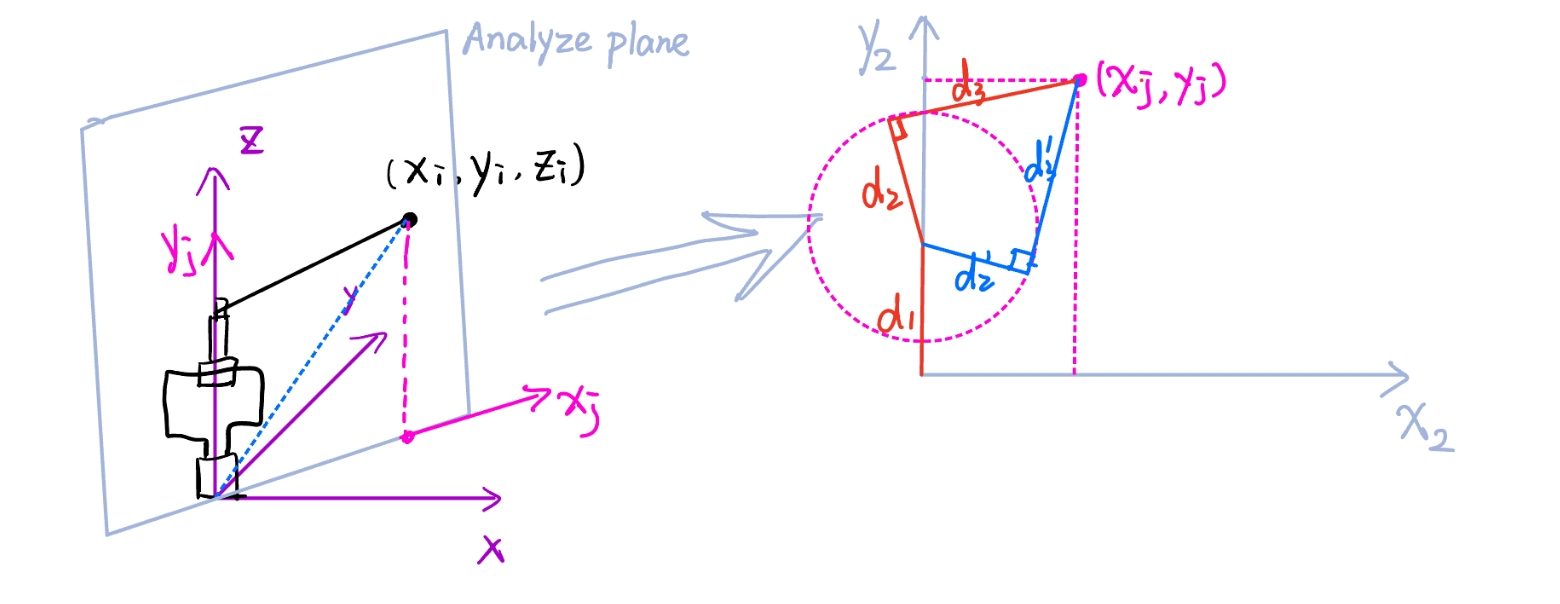
\includegraphics[width=0.8\textwidth]{Image/2.png}
	\caption{RRP机器人工作空间示意图}
\end{figure}

如果轨迹点在此圆外,那么会有两个解(如上图所示),如果在圆上,那么就会有一个解$d_3=0$,如果在圆内,就没有解。

\section{6R机械臂运动学分析}
\subsection{建立MDH坐标系,并填写表格}

建立的MDH坐标系如下:
\begin{figure}[h]
	\centering
	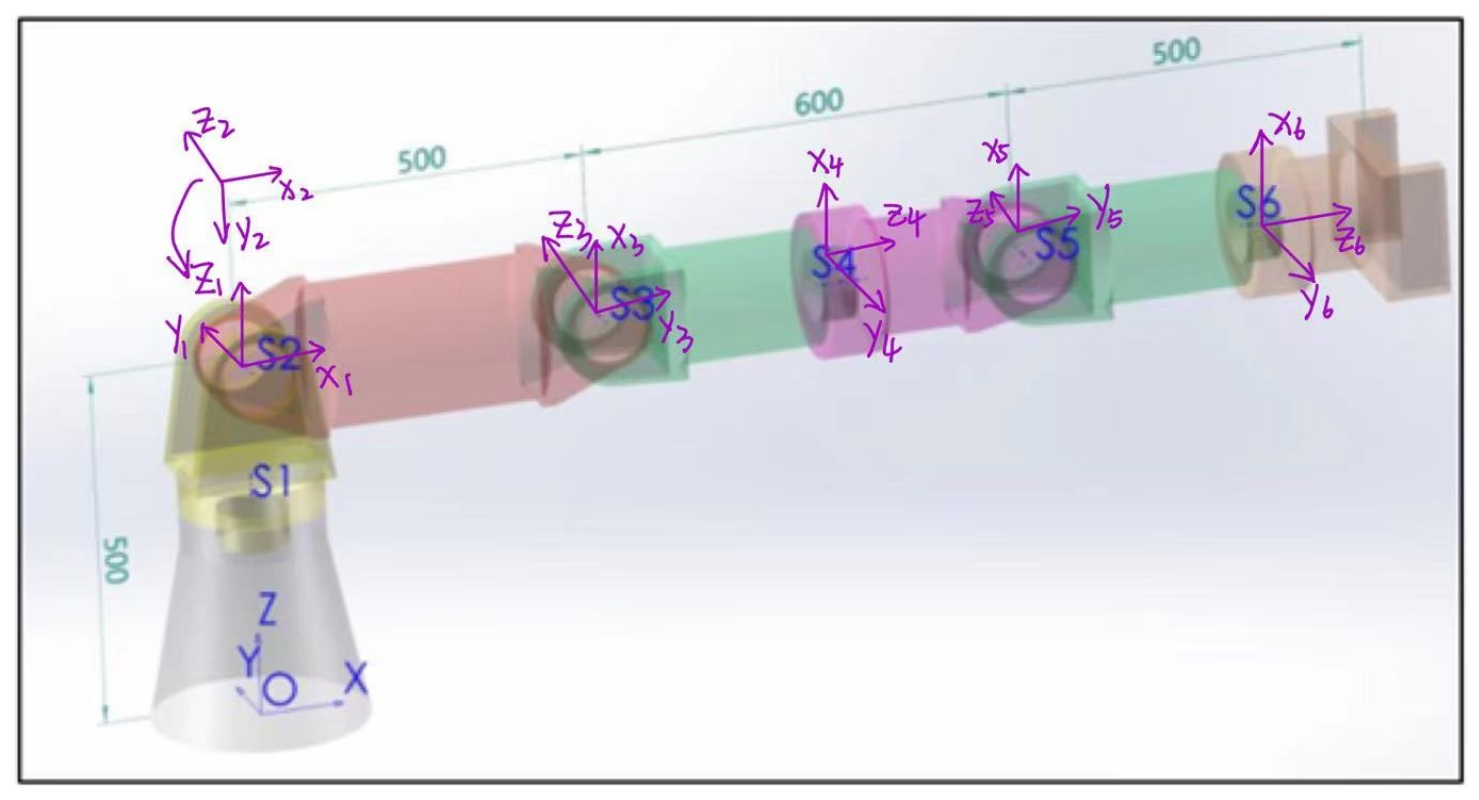
\includegraphics[width=0.7\textwidth]{Image/3.png}
	\caption{6R机器人建系示意图}
\end{figure}

根据建立的坐标系,填写以下表格:

\begin{table}[h]
	\centering
	\setlength{\tabcolsep}{4mm}{
	\begin{tabular}{
	>{\columncolor[HTML]{DAE8FC}}c |
	>{\columncolor[HTML]{DAE8FC}}c |
	>{\columncolor[HTML]{DAE8FC}}c |
	>{\columncolor[HTML]{DAE8FC}}c |
	>{\columncolor[HTML]{DAE8FC}}c |
	>{\columncolor[HTML]{DAE8FC}}c |
	>{\columncolor[HTML]{DAE8FC}}c }
	\hline\hline
	\diagbox{Parameter}{Joints}		 & 1           & 2           & 3             & 4            & 5            & 6            \\ \hline
	$\theta$ & $\theta_1+0$ & $\theta_2+0$ & $\theta_3-90$ & $\theta_4+0$ & $\theta_5+0$ & $\theta_6+0$ \\ \hline
	$d$      & 500         & 0           & 0             & 600          & 0            & 500          \\ \hline
	$\alpha_{i-1}$ & 0           & -90          & 0             & -90          & 90           & -90           \\ \hline
	$a_{i-1}$      & 0           & 0           & 500           & 0            & 0            & 0            \\ \hline\hline
	\end{tabular}}
	\caption{6R机器人MDH参数表}
	\end{table}

\subsection{写出 DH 矩阵,并使用 DH 矩阵表示机构末端相对于基座的位姿(不必写出累乘的结果)}
由题意,逐步分析每个关节的David-Hartenberg参数:

\begin{itemize}
	\item Joint1: $\theta = \theta_1$,$a_0=0$,$d_1=500$,$\alpha_0=0$,$^0R_1=\begin{bmatrix}
		\cos\theta_1 & -\sin\theta_1 & 0 & 0 \\
		\sin\theta_1 & \cos\theta_1 & 0 & 0 \\
		0 & 0 & 1 & 500 \\
		0 & 0 & 0 & 1
	\end{bmatrix}$
	\item Joint2: $\theta = \theta_2$,$a_1=0$,$d_2=0$,$\alpha_1=-90$,$^1R_2=\begin{bmatrix}
		\cos\theta_2 & -\sin\theta_2 & 0 & 0 \\
		0 & 0 & 1 & 0 \\
		-\sin\theta_2 & -\cos\theta_2 & 0 & 0 \\
		0 & 0 & 0 & 1
	\end{bmatrix}$
	\item Joint3: $\theta = \theta_3-90^\circ$,$a_2=500$,$d_3=0$,$\alpha_2=0$,$^2R_3=\begin{bmatrix}
		\cos(\theta_3-90) & -\sin(\theta_3-90) & 0 & 500 \\
		\sin(\theta_3-90) & \cos(\theta_3-90) & 0 & 0 \\
		0 & 0 & 1 & 0 \\
		0 & 0 & 0 & 1
	\end{bmatrix}$
	\item Joint4: $\theta = \theta_4$,$a_3=0$,$d_4=600$,$\alpha_3=-90$,$^3R_4=\begin{bmatrix}
		\cos\theta_4 & -\sin\theta_4 & 0 & 0 \\
		0 & 0 & 1 & 600 \\
		-\sin\theta_4 & -\cos\theta_4 & 0 & 0 \\
		0 & 0 & 0 & 1
	\end{bmatrix}$
	\item Joint5: $\theta = \theta_5$,$a_4=0$,$d_5=0$,$\alpha_4=90$,$^4R_5=\begin{bmatrix}
		\cos\theta_5 & -\sin\theta_5 & 0 & 0 \\
		0 & 0 & -1 & 0 \\
		\sin\theta_5 & \cos\theta_5 & 0 & 0 \\
		0 & 0 & 0 & 1
	\end{bmatrix}$
	\item Joint6: $\theta = \theta_6$,$a_5=0$,$d_6=500$,$\alpha_5=-90$,$^5R_6=\begin{bmatrix}
		\cos\theta_6 & -\sin\theta_6 & 0 & 0 \\
		0 & 0 & 1 & 500 \\
		-\sin\theta_6 & -\cos\theta_6 & 0 & 0 \\
		0 & 0 & 0 & 1
	\end{bmatrix}$
\end{itemize}

由DH参数的定义是在动坐标系上的,所以我们需要将这些矩阵进行累右乘,得到机构末端相对于基座的位姿。
$$
^0T_6=^0R_1(\theta_1) ^1R_2(\theta_2) ^2R_3(\theta_3) ^3R_4(\theta_4) ^4R_5(\theta_5) ^5R_6(\theta_6)
$$

具体的累乘结果不用表述。

\subsection{使用 Robotics 工具箱建立该机构的运动学模型, 使得$\theta_i=0$时,机构位形如图2
所示}

\href{src/Rhw_3_2_2_main.m}{Click here to jump to the MATLAB code.}

在本代码中我建立了机械臂后运行示教模式,可以得到下图所示的初始状态,即$\theta_i=0$时,机构位形如图4所示。
\begin{figure}[h]
	\centering
	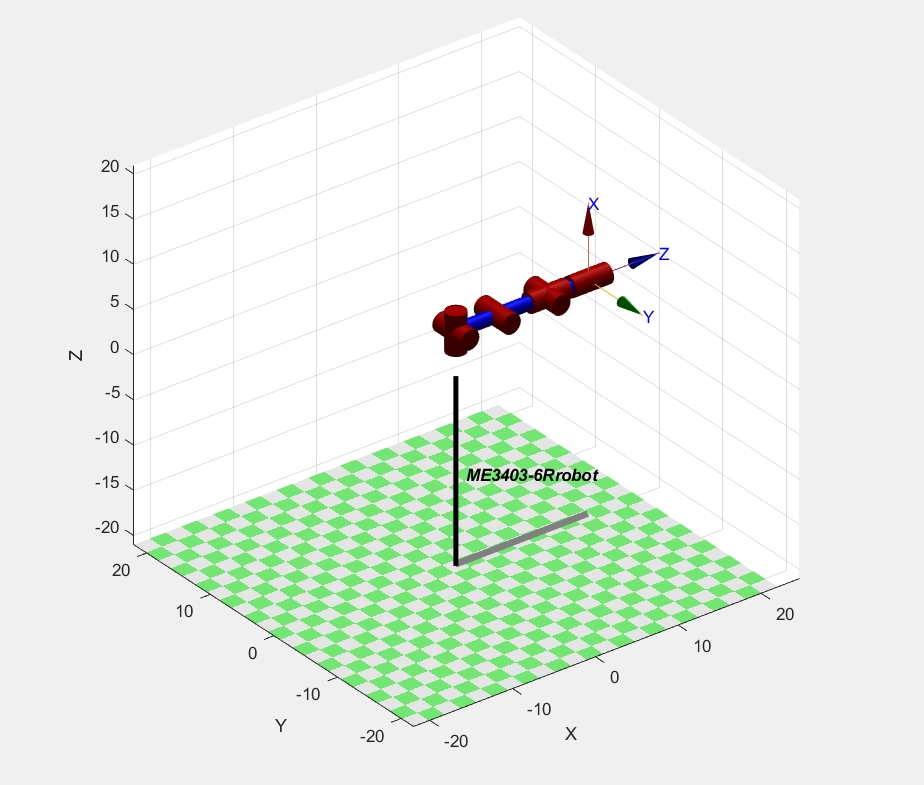
\includegraphics[width=0.6\textwidth]{Image/4.png}
	\caption{MATLAB中建立的模型并确定其初始位姿}
\end{figure}

通过示教模式改变六个参数角度可以得到对应的机构位形。

\subsection{推导实现该机构的逆运动学求解(使用解析法,求出所有可能的解),并使用如下结果和robotics 工具箱函数 ikine 校验编程结果。}
[Notice]尽我可能做到最后。

根据第二问的结果,注意到$^3T_5$这个矩阵的第四列元素是定的,因此可以从这个角度入手解决逆运动学的解析解。

首先,不妨设最终的位姿表达式(NOA)形式为
\begin{equation}
	^0T_6=\begin{bmatrix}
		\mathbf{n} & \mathbf{o} & \mathbf{a} & \mathbf{p} \\
		0 & 0 & 0 & 1
	\end{bmatrix}
	=
	\begin{bmatrix}
		n_x & o_x & a_x & p_x \\
		n_y & o_y & a_y & p_y \\
		n_z & o_z & a_z & p_z \\
		0 & 0 & 0 & 1
	\end{bmatrix}
\end{equation}

对于$^3T_5$:

\begin{equation}
	\begin{aligned}
	^3T_5=^3T_4^4T_5&=\begin{bmatrix}
		\cos\theta_4 & -\sin\theta_4 & 0 & 0 \\
		0 & 0 & 1 & 6 \\
		-\sin\theta_4 & -\cos\theta_4 & 0 & 0 \\
		0 & 0 & 0 & 1
	\end{bmatrix}\begin{bmatrix}
		\cos\theta_5 & -\sin\theta_5 & 0 & 0 \\
		0 & 0 & -1 & 0 \\
		\sin\theta_5 & \cos\theta_5 & 0 & 0 \\
		0 & 0 & 0 & 1
	\end{bmatrix}\\
	&=\begin{bmatrix}
		c_4c_5 & -c_4s_5 & s_4 & 0 \\
		s_5 & c_5 & 0 & 6\\
		-s_4c_5 & s_4s_5 & c_4 & 0 \\
		0 & 0 & 0 & 1
	\end{bmatrix}
	\end{aligned}
\end{equation}

又由于$^0T_6=(^0T_3)(^3T_5)(^5T_6)$,由矩阵乘法的性质,$^3T_5=(^0T_3)^{-1}(^0T_6)(^5T_6)^{-1}$,而

\begin{equation}
	\begin{aligned}
		^0T_3&=^0T_1^1T_2^2T_3\\
		&=\begin{bmatrix}
			\cos\theta_1 & -\sin\theta_1 & 0 & 0 \\
			\sin\theta_1 & \cos\theta_1 & 0 & 0 \\
			0 & 0 & 1 & 5 \\
			0 & 0 & 0 & 1
		\end{bmatrix}\begin{bmatrix}
			\cos\theta_2 & -\sin\theta_2 & 0 & 0 \\
			0 & 0 & 1 & 0 \\
			-\sin\theta_2 & -\cos\theta_2 & 0 & 0 \\
			0 & 0 & 0 & 1
		\end{bmatrix}\begin{bmatrix}
			\cos\theta_3 & -\sin\theta_3 & 0 & 5 \\
			\sin\theta_3 & \cos\theta_3 & 0 & 0 \\
			0 & 0 & 1 & 0 \\
			0 & 0 & 0 & 1	
		\end{bmatrix}\\
		&=\begin{bmatrix}
			c_1c_2c_3-c_1s_2s_3 & -c_1c_2s_3-c_1s_2c_3 & -s_1 & 5c_1c_2 \\
			s_1c_2c_3-s_1s_2s_3 & -s_1c_2s_3-s_1s_2c_3 & c_1 & 5s_1c_2 \\
			-s_2c_3-c_2s_3 & s_2s_3-c_2c_3 & 0 & 5s_2 \\
			0 & 0 & 0 & 1
		\end{bmatrix}
	\end{aligned}
\end{equation}

由三角函数展开公式
$$
cos(\alpha\pm\beta)=cos\alpha cos\beta\mp sin\alpha sin\beta,sin(\alpha\pm\beta)=sin\alpha cos\beta\pm cos\alpha sin\beta
$$

记$cos\theta_1=c_1,sin(\theta_1+\theta_2)=s_{12},cos(\theta_1+\theta_2+\theta_3)=c_{123}$,以此类推,可简化上述$^0T_3$的表达式:

\begin{equation}
	\begin{aligned}
		^0T_3&=\begin{bmatrix}
			c_{1}c_{23} & -c_{1}s_{23} & -s_1 & 5c_1c_2 \\
			s_{1}c_{23} & -s_{1}s_{23} & c_1 & 5s_1c_2 \\
			-s_{23} & -c_{23} & 0 & -5s_2 \\
			0 & 0 & 0 & 1
		\end{bmatrix}
	\end{aligned}
\end{equation}

由Chapter2数学基础中的快捷求逆的方法,可以知道

\begin{equation}
	\begin{aligned}
		^0T_3^{-1}&=\begin{bmatrix}
			^0R_3^T & -^0R_3^T\mathbf{p}_3 \\
			0 & 1
		\end{bmatrix}=
		\begin{bmatrix}
			c_1c_{23} & s_{1}c_{23} & -s_{23} & -5c_3 \\
			-c_1s_{23} & -s_1s_{23} & -c_{23} & 5s_3 \\
			-s_1 & c_1 & 0 & 0 \\
			0 & 0 & 0 & 1
			\end{bmatrix}
	\end{aligned}
\end{equation}

至于第四列是如何得到的,我们能够很惊讶地发现:
\begin{equation}
	\begin{aligned}
	-^0R_3^T\mathbf{p}_3&=\begin{bmatrix}
		-c_1c_{23} & -s_{1}c_{23} & s_{23} \\
		c_1s_{23} & s_1s_{23} & c_{23} \\
		s_1 & -c_1 & 0
	\end{bmatrix}\begin{bmatrix}
		5c_1c_2 \\
		5s_1c_2 \\
		-5s_2
	\end{bmatrix}=\begin{bmatrix}
		-5c2c_{23}-5s_2s_{23} \\
		5c_2s_{23}-5s_2c_{23} \\
		0
	\end{bmatrix}\\
	&=\begin{bmatrix}
		-5cos(\theta_2+\theta_3-\theta_2) \\
		5sin(\theta_2+\theta_3-\theta_2) \\
		0
	\end{bmatrix}=
	\begin{bmatrix}
		-5c_3 \\
		5s_3 \\
		0
	\end{bmatrix}
	\end{aligned}
\end{equation}

同理我们接着用上面的公式求取$^5T_6$的逆矩阵,即:

\begin{equation}
	\begin{aligned}
		^5T_6^{-1}&=\begin{bmatrix}
			^5R_6^T & -^5R_6^T\mathbf{p}_6 \\
			0 & 1
		\end{bmatrix}=
		\begin{bmatrix}
			c_6 & 0 & -s_6 & 0 \\
			-s_6 & 0 & -c_6 & 0 \\
			0 & 1 & 0 & -5 \\
			0 & 0 & 0 & 1
			\end{bmatrix}
	\end{aligned}
\end{equation}

至此,我们做好了准备工作,可以开始求解逆运动学解了。(后面有点算晕了)

\begin{equation}
	\begin{aligned}
		^3T_5&=(^0T_3)^{-1}(^0T_6)(^5T_6)^{-1}
		=\begin{bmatrix}
			c_4c_5 & -c_4s_5 & s_4 & 0 \\
			s_5 & c_5 & 0 & \textcolor{red}{6}\\
			-s_4c_5 & s_4s_5 & c_4 & 0 \\
			0 & 0 & 0 & 1
		\end{bmatrix}
	\end{aligned}
\end{equation}

注意到第二行第四列元素是一个\textbf{常数}!这意味着我们可以从这里切入解出某些角度,不过计算的时候我们可以观察矩阵形式,投机取巧,避免一些不必要的计算量:
\begin{equation}
	\begin{aligned}
		^3T_5&=(^0T_3)^{-1}(^0T_6)(^5T_6)^{-1}\\
		&=\begin{bmatrix}
			* & * & * & * \\
			-c_1s_{23} & -s_1s_{23} & -c_{23} & 5s_3 \\
			* & * & * & * \\
			* & * & * & *
		\end{bmatrix}
		\begin{bmatrix}
			n_x & o_x & a_x & p_x \\
			n_y & o_y & a_y & p_y \\
			n_z & o_z & a_z & p_z \\
			0 & 0 & 0 & 1
		\end{bmatrix}
		\begin{bmatrix}
			* & * & * & 0\\
			* & * & * & 0\\
			* & * & * & -5\\
			0 & 0 & 0 & 1
		\end{bmatrix}\\
		&=
		\begin{bmatrix}
			* & * & * & * \\
			* & * & -c_1s_{23}a_x-s_1s_{23}a_y-c_{23}a_z &  \parbox{3cm}{ $c_1s_{23}p_x-s_1c_{23}p_y\\-c_{23}p_z+5s_3$} \\
			* & * & * & * \\
			* & * & * & *
		\end{bmatrix}
		\begin{bmatrix}
			* & * & * & 0\\
			* & * & * & 0\\
			* & * & * & -5\\
			* & * & * & 1\\
		\end{bmatrix}\\
		&=\begin{bmatrix}
			* & * & * & * \\
			* & * & *& (5a_x-p_x)c_1s_{23}+(5a_y-p_y)s_1s_{23}+(5a_z-p_z)c_{23}+5s_3 \\
			* & * & * & * \\
			* & * & * & *
		\end{bmatrix}
	\end{aligned}
\end{equation}

上述表达式中的'*'代表的是一些不重要的项,即矩阵乘法的过程中对结果的第四列元素不产生影响、或是因为存在‘0’元素导致相乘结果为0,不必详细计算的项。

所以
$$
(5a_x-p_x)c_1s_{23}+(5a_y-p_y)s_1s_{23}+(5a_z-p_z)c_{23}+5s_3=6
$$

同样的做法我们考察$^3T_5$的第三行第四列元素,可以得到:
$$
-5s_1a_x-5c_1a_y+c_1p_y-s_1p_x=0
$$

上面这个方程就非常关键了,因为它仅是关于$\theta_1$的方程,我们可以通过这个方程解出$\theta_1$的值:
$$
let \quad m=p_x-5a_x,n=p_y-5a_y
$$
$$
nc_1-ms_1=0
$$

由第一章的知识:
$$
\theta_1 = Atan2(m,n)
$$

有了$\theta_1$的值,我们可以继续求解代入上面的方程(加上第一行第四列元素的方程)求解$\theta_2,\theta_3$的值。$\theta_4,\theta_5,\theta_6$同理。

当然我写到这里已经是使尽了浑身解数。不得不说我现在的数学基础和运算能力还不足以支撑我完成这项艰巨而复杂的解析解任务。我参考了一些资料,使用了Pieper的解法,可能还是不太行,希望以后有时间可以再多多研究一下。
\href{src/Rhw_3_2_3_main.m}{Click here to jump to the MATLAB code.}
\end{document}

